%%%%%%%%%%%%%%%%%%%%%%%%%%%%%%%%%%%%%%%%%
% Beamer Presentation
% LaTeX Template
% Version 1.0 (10/11/12)
%
% This template has been downloaded from:
% http://www.LaTeXTemplates.com
%
% License:
% CC BY-NC-SA 3.0 (http://creativecommons.org/licenses/by-nc-sa/3.0/)
%
%%%%%%%%%%%%%%%%%%%%%%%%%%%%%%%%%%%%%%%%%

%----------------------------------------------------------------------------------------
%	PACKAGES AND THEMES
%----------------------------------------------------------------------------------------

\documentclass[xcolor={dvipsnames}]{beamer}

\mode<presentation> {

% The Beamer class comes with a number of default slide themes
% which change the colors and layouts of slides. Below this is a list
% of all the themes, uncomment each in turn to see what they look like.

%\usetheme{default}
%\usetheme{AnnArbor}
%\usetheme{Antibes}
%\usetheme{Bergen}
%\usetheme{Berkeley}
%\usetheme{Berlin}
%\usetheme{Boadilla}
%\usetheme{CambridgeUS}
%\usetheme{Copenhagen}
%\usetheme{Darmstadt}
%\usetheme{Dresden}
\usetheme{Frankfurt}
%\usetheme{Goettingen}
%\usetheme{Hannover}
%\usetheme{Ilmenau}
%\usetheme{JuanLesPins}
%\usetheme{Luebeck}
%\usetheme{Madrid}
%\usetheme{Malmoe}
%\usetheme{Marburg}
%\usetheme{Montpellier}
%\usetheme{PaloAlto}
%\usetheme{Pittsburgh}
%\usetheme{Rochester}
%\usetheme{Singapore}
%\usetheme{Szeged}
%\usetheme{Warsaw}

% As well as themes, the Beamer class has a number of color themes
% for any slide theme. Uncomment each of these in turn to see how it
% changes the colors of your current slide theme.

%\usecolortheme{albatross}
%\usecolortheme{beaver}
%\usecolortheme{beetle}
%\usecolortheme{crane}
%\usecolortheme{dolphin}
%\usecolortheme{dove}
%\usecolortheme{fly}
%\usecolortheme{lily}
%\usecolortheme{orchid}
%\usecolortheme{rose}
%\usecolortheme{seagull}
%\usecolortheme{seahorse}
%\usecolortheme{whale}
%\usecolortheme{wolverine}

%\setbeamertemplate{footline} % To remove the footer line in all slides uncomment this line
%\setbeamertemplate{footline}[page number] % To replace the footer line in all slides with a simple slide count uncomment this line

%\setbeamertemplate{navigation symbols}{} % To remove the navigation symbols from the bottom of all slides uncomment this line
}

\usepackage{graphicx} % Allows including images
\usepackage{booktabs} % Allows the use of \toprule, \midrule and \bottomrule in tables
\usepackage{multimedia}
\usepackage{pgfplots}
\usepackage{tikz}
\usetikzlibrary{shapes.geometric, arrows}

\usepackage{soul}

\makeatletter
\newcommand\SoulColor{%
  \let\set@color\beamerorig@set@color
  \let\reset@color\beamerorig@reset@color}
\makeatother

\newcommand{\hlc}[2][yellow]{ {\sethlcolor{#1} \SoulColor\hl{#2}} }
\usepackage{color}

%----------------------------------------------------------------------------------------
%	TITLE PAGE
%----------------------------------------------------------------------------------------

\title[Dynamic Resource Allocation]{Dynamic Resource Allocation for Multi-Camera Systems} % The short title appears at the bottom of every slide, the full title is only on the title page

\author{Eugenio Bargiacchi} % Your name
\institute[UvA] % Your institution as it will appear on the bottom of every slide, may be shorthand to save space
{
University of Amsterdam \\ % Your institution for the title page
\medskip
\textit{svalorzen@gmail.com} % Your email address
}
\date{16 March, 2016} % Date, can be changed to a custom date

\begin{document}

\begin{frame}
\titlepage % Print the title page as the first slide
\end{frame}

\begin{frame}
\frametitle{Overview} % Table of contents slide, comment this block out to remove it
\tableofcontents % Throughout your presentation, if you choose to use \section{} and \subsection{} commands, these will automatically be printed on this slide as an overview of your presentation
\end{frame}

%----------------------------------------------------------------------------------------
%	PRESENTATION SLIDES
%----------------------------------------------------------------------------------------

\section{Introduction}

\subsection{The Problem}
\begin{frame}
\frametitle{Resourse Constraints in Multi-Camera Systems}

\begin{block}{}
Camera systems are now everywhere. \\
Cheaper than ever before.
\end{block}
\begin{block}{}
Increasing operational costs as size increases:
\begin{itemize}
\item Electricity
\item Bandwidth
\item Coverage
\item Computation
\item Storage
\end{itemize}
\end{block}
\end{frame}

\begin{frame}
Can we do this more efficiently?
\end{frame}

\subsection{Active Perception}
\begin{frame}
\frametitle{Active Perception}
\begin{block}{Active Perception}
\textit{A task where a decision making entity called agent, subject to resource
constraints, needs to take actions in order to reduce some form of uncertainty about a particular
target environment.}
\end{block}
\end{frame}

%------------------------------------------------
\section{Background} % Sections can be created in order to organize your presentation into discrete blocks, all sections and subsections are automatically printed in the table of contents as an overview of the talk
%------------------------------------------------

\subsection{Partially Observable Markov Decision Processes}

\begin{frame}
\frametitle{POMDP}
\begin{block}{}
Agent acts upon an \textit{environment}.  \\~\\
Obtains \textit{observations} and \textit{reward}. \\~\\
The environment \textit{transitions} to a new state afterwards.
\end{block}
\end{frame}

\begin{frame}
\frametitle{POMDP network}
\begin{figure}
\centerline{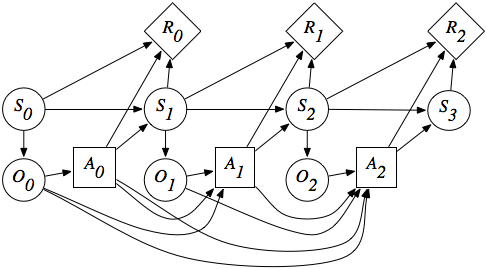
\includegraphics[height=6cm]{images/pomdp.png}}
\caption{From \textit{http://www.cs.ubc.ca/~kooshakh/research.html}}
\end{figure}
\end{frame}

\begin{frame}
\frametitle{Formal Definition}
\begin{block}{POMDP}
\begin{equation}
 POMDP = <S,A,T,R,\Omega,O,h> \nonumber
\end{equation}
\end{block}
\begin{block}{Horizon ($h$)}
    Defines the number of timesteps the agent is going to plan in advance for.
\end{block}
\begin{block}{State space ($S$)}
    Defines all the states that the environment can ever be.
\end{block}
\begin{block}{Action space ($A$)}
    Defines all the actions that the agent can take.
\end{block}
\begin{block}{Observation space ($\Omega$)}
    Defines all the observations that the agent can obtain.
\end{block}
\end{frame}

\begin{frame}
\frametitle{$T$ and $O$}
\begin{block}{Transition function ($T$)}
    Defines the probability of happening for each possible transition from state to state.
\end{block}
\begin{block}{Observation function ($O$)}
    Defines the probability of obtaining a certain observation from a state and action.
\end{block}
\end{frame}

\begin{frame}
\frametitle{How do we keep track of the state?}
\centerline{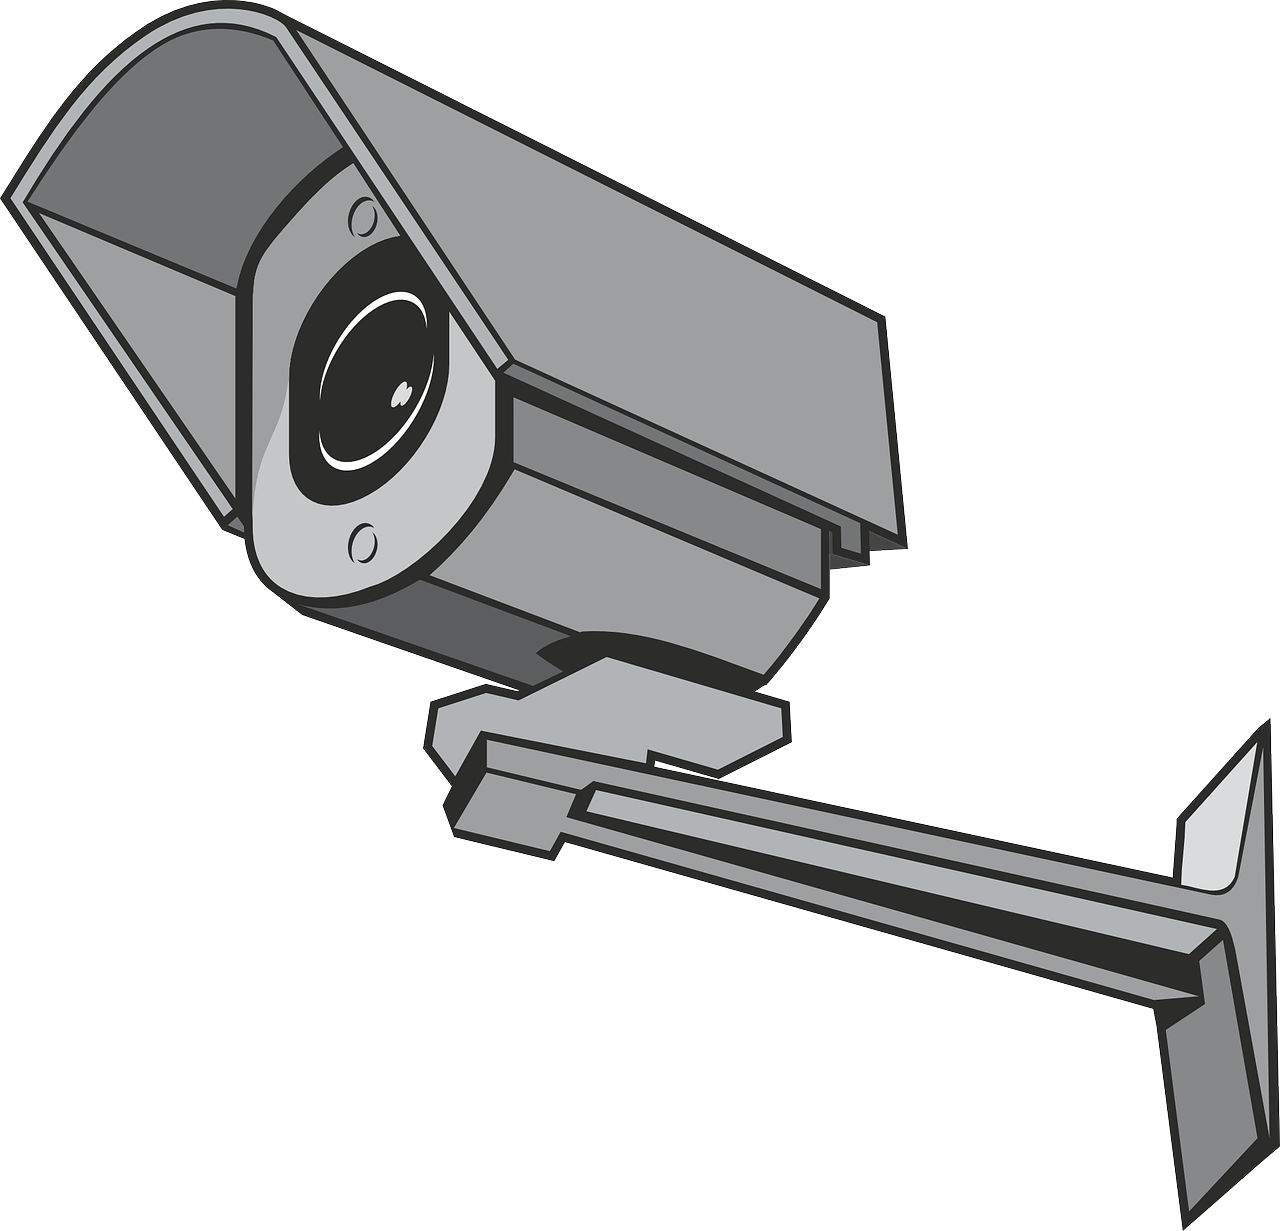
\includegraphics[height=6cm]{images/camera.png}}
\end{frame}

\begin{frame}
\frametitle{Belief}
\begin{equation}
 b'(s') = \frac{O(s', a, o)\sum_{s\in S}T(s,a,s')b(s)}{Pr(o|a,b)} \nonumber
\end{equation}
\end{frame}

\begin{frame}
\frametitle{Belief}
\begin{center}
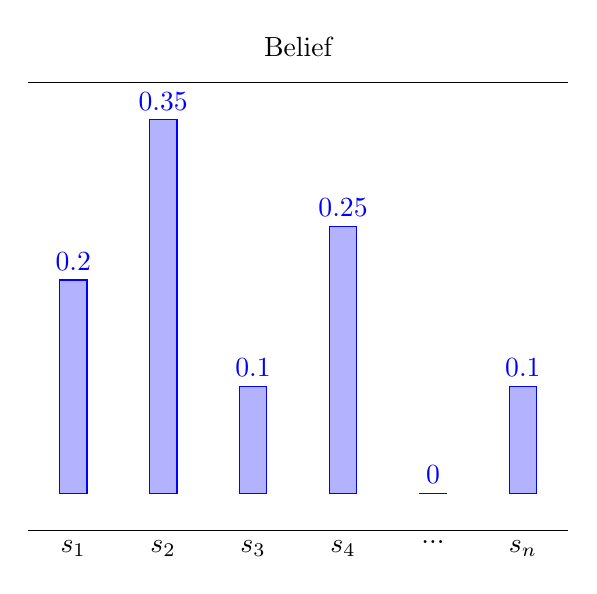
\begin{tikzpicture}
  \begin{axis}[title  = Belief,
    ybar,
    axis y line       = none,
    xtick = data,
    tickwidth         = 0pt,
    symbolic x coords = {$s_1$, $s_2$, $s_3$, $s_4$, ..., $s_n$},
    nodes near coords,
  ]
  \addplot coordinates { ($s_1$, 0.2) ($s_2$, 0.35)
                         ($s_3$, 0.1)  ($s_4$, 0.25)
                         (..., 0.0) ($s_n$, 0.1)};
  \end{axis}
\end{tikzpicture}
\end{center}
\end{frame}

\subsection{$\rho$POMDP}

\begin{frame}
\frametitle{Reward Function}
\begin{block}{Reward function ($R$)}
    Defines the reward obtained during specific state transitions.
\end{block}
\begin{block}{Belief-dependent Reward Function ($\rho$)}
    Defines the reward obtained during specific belief transitions.
\end{block}
\begin{block}{$\rho$POMDP}
    A POMDP that uses $\rho$ rather than $R$.
\end{block}
\end{frame}
%------------------------------------------------

\begin{frame}
\frametitle{Policies}
\begin{block}{Objectives}
Maximize \textit{expected reward}:
\begin{equation}
 \mathbb{E}[\text{return}] = \mathbb{E} \left [ \sum_{t=0}^{h-1} R(s_t, a_t, s_{t+1}) \right ] \nonumber
\end{equation}
\end{block}
\end{frame}

\begin{frame}
\frametitle{Planning Problems with $\rho$}
\begin{block}{}
How to plan for infinite beliefs? We need infinite plans!
\end{block}
\begin{block}{}
Possible approach is to approximate $rho$. Then we have a finite number of possibilities to take
into account.
\end{block}
\begin{block}{}
Other approach is to plan online. We plan during real execution, only for the current belief. No
more infinities.
\end{block}
\end{frame}

%------------------------------------------------

\section[MCTS]{Monte Carlo Tree Search}
\subsection{Online Planning in MDPs}
\begin{frame}
\frametitle{Monte Carlo Tree Search}
\begin{block}{}
Very fast approximate online algorithm. \\~\\
Originally conceived for Go (and the base for AlphaGo!). \\~\\
Only requires a black box simulator of the environment. \\~\\
Can handle very large state spaces.
\end{block}
\end{frame}

\begin{frame}
\frametitle{MCTS Algorithm}
\centerline{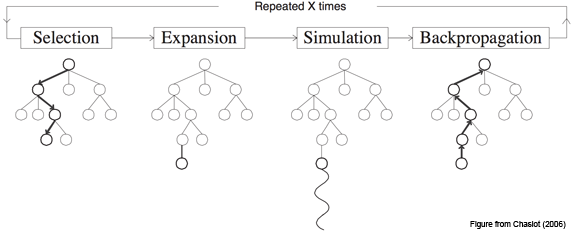
\includegraphics[height=5cm]{images/mcts.png}}
\end{frame}

\section[POMCP]{Partially Observable Monte Carlo Planning}
\subsection{Online Planning in POMDPs}
\begin{frame}
\frametitle{Partially Observable Monte Carlo Planning}
\begin{block}{}
MCTS \textit{could} work with POMDPs, but belief updates are expensive. \\~\\
POMCP extends MCTS in order to allow partially obserable states. \\~\\
Approximates beliefs using particles, to avoid expensive updates.
\end{block}
\end{frame}

\begin{frame}
\frametitle{POMCP Algorithm}
\begin{figure}[ht!]
\centering
\resizebox{!}{6cm}{%
\begin{tikzpicture}[->,>=stealth',shorten >=1pt,auto,node distance=4cm,thick,main node/.style={circle,draw,font=\Large\bfseries}]
\tikzstyle{state} = [circle, minimum size=.7cm, draw=black, fill=green!30]
\tikzstyle{empty} = [coordinate,draw=none, fill=none]
\tikzstyle{arrow} = [thick,->,>=stealth]

\node (particleb) at (0,.8) [draw=none] {[\hlc[Yellow]{$s_1$},$s_2$,...,$s_k$]};
\node (b)  at (0,0)  [state] {$b$};
\node (a1) at (0,-2) [empty] {};
\node (a2) at (1.5,-2) [empty] {};
\node (a3) at (3,-2) [empty] {};
\node (a4) at (4.5,-2) [empty] {};
\node (b1) at (0,-5) [state] {$b'$};
\node (b2) at (1.5,-5) [state] { };
\node (b3) at (3,-5) [state] { };
\node (b4) at (4.5,-5) [state] { };
\node (particleb1) at (0,-5.8) [draw=none] {[\hlc[Yellow]{$s'$},...]};
\node (g) at (-2.2,-2.3) [draw=none,rotate=90] {$G(s,a)$};
\node (null) at (0, -7.1) [draw=none, minimum width=1.35cm, minimum height=.5cm] {  ...  };
\node (roll) at (0, -8.1) [draw=none] {Rollout};

\path
     (b)  edge [] node [left,pos=0.7] (aa) {\hlc[Dandelion]{$a_1$}} (a1)
          edge [] node [left,pos=0.7] {$a_2$} (a2)
          edge [] node [left,pos=0.7] {$a_3$} (a3)
          edge [dashed] node {} (a4)
     (a1) edge [] node [left,pos=0.6] (oo) {\hlc[SkyBlue]{$o_1$}} (b1)
          edge [] node [left,pos=0.6] {$o_2$} (b2)
          edge [] node [left,pos=0.6] {$o_3$} (b3)
          edge [dashed] node {} (b4)
     (particleb1) edge (null)
     (null) edge (roll);

\draw [draw=none] (b1) -- node [pos=0.6] (tmpx) {} (oo);
\draw [draw=none] (g.south |- tmpx) -- node [midway] (tmp) {} (tmpx);

\draw (null) -| (tmp);
\draw (roll) -| (tmp);
\draw (b1 -| tmp.south) -- (b1);

\draw [-,line width=5pt,draw=white] (g.south) |- (particleb1);

\draw (g.south |- tmp.south) -- (tmp.south) |- node [below,pos=0.2,rotate=90] {\hlc[LimeGreen]{ $r$ }} (b);
\draw [-,line width=5pt,draw=white] (g.south) |- (oo);
\draw [*->,draw=black] (g.south) |- (oo);

\draw (g.south) |- (particleb1);

\draw [-,line width=5pt,draw=white] (aa) -| (g.south);
\draw (aa) -| (g.south);
\draw [draw=black] (particleb) -| (g.south);

\end{tikzpicture}
}
\end{figure}
\end{frame}

\section{$\rho$POMCP}
\subsection{Problems}
\begin{frame}
\frametitle{$\rho$POMCP}
\begin{block}{}
POMCP cannot directly handle belief based reward functions. \\~\\
How to compute $\rho$ on particle beliefs? \\~\\
How to update estimates of $\rho$ back in the tree?
\end{block}
\end{frame}

\subsection{Reward Function Estimation}
\begin{frame}
\frametitle{Estimating $\rho$}
\begin{block}{Max of Belief}
Maximum likelihood approximation:
\begin{equation}
N(max_s)/N(b) \nonumber
\end{equation}
\end{block}

\begin{block}{Entropy}
Ideal approximation:
\begin{equation}
-\hat{H}(b) \approx \sum_s \frac{N(s)}{N} \log \frac{N(s)}{N} \nonumber
\end{equation}
For large particle beliefs this would require recomputing too many terms.
Instead we only recompute the last one:
\begin{equation}
-\hat{H}(b) \approx -\hat{H}_{old}(b) - \frac{N(s)}{N} \log \frac{N(s)}{N} + \frac{N(s)+1}{N+1} \log \frac{N(s)+1}{N+1}  \nonumber
\end{equation}
\end{block}
\end{frame}

\subsection{Backpropagating Rewards}
\begin{frame}
\frametitle{Reward Backpropagation}
\begin{block}{}
Both in MCTS and POMCP, rewards are sampled from $R$ \\~\\
All rewards obtained this way are valid, and they are averaged together.
\end{block}
\begin{block}{}
$\rho$POMCP does not sample rewards! \\~\\
Need a way to backpropagate estimates as they change, revising previous values. \\~\\
Must revise only estimates for specific child observations!
\end{block}
\end{frame}

\begin{frame}
\frametitle{Reward Backpropagation}
\begin{block}{}
We keep the mechanism of averaging rewards, but we pass crafted rewards.
\begin{equation}
n_{\tilde{o}}(r'_{\tilde{o}} - r_{\tilde{o}}) + r'_{\tilde{o}} \nonumber
\end{equation}
The end result is that the new average will be equal to our new estimation.
\begin{equation}
\rho(b,a) \approx \frac{\sum_{o\in\Omega} n_o r_o}{N} \approx \frac{ n_{\tilde{o}} r_{\tilde{o}} + \sum_{o \neq \tilde{o} \in \Omega} n_o r_o}{N} \nonumber
\end{equation}
\begin{equation}
\rho(b,a) \approx \frac{ n_{\tilde{o}} r_{\tilde{o}} + n_{\tilde{o}}(r'_{\tilde{o}} - r_{\tilde{o}}) + r'_{\tilde{o}} + \sum_{o \neq \tilde{o} \in \Omega} n_o r_o}{N+1} \nonumber
\end{equation}
\begin{equation}
\rho(b,a) \approx \frac{ ( n_{\tilde{o}}+1) r'_{\tilde{o}} + \sum_{o \neq \tilde{o} \in \Omega} n_o r_o}{N+1} \nonumber
\end{equation}
\end{block}
\end{frame}

\begin{frame}
\frametitle{$\rho$POMCP Algorithm}
\begin{figure}[ht!]
\centering
\resizebox{!}{6cm}{%
\begin{tikzpicture}[->,>=stealth',shorten >=1pt,auto,node distance=4cm,thick,main node/.style={circle,draw,font=\Large\bfseries}]
\tikzstyle{state} = [circle, minimum size=.7cm, draw=black, fill=green!30]
\tikzstyle{empty} = [coordinate,draw=none, fill=none]
\tikzstyle{arrow} = [thick,->,>=stealth]

\node (particleb) at (0,.8) [draw=none] {[\hlc[Yellow]{$s_1$},$s_2$,...,$s_k$]};
\node (b)  at (0,0)  [state] {$b$};
\node (a1) at (0,-2) [empty] {};
\node (a2) at (1.5,-2) [empty] {};
\node (a3) at (3,-2) [empty] {};
\node (a4) at (4.5,-2) [empty] {};
\node (b1) at (0,-5) [state] {$b'$};
\node (b2) at (1.5,-5) [state] { };
\node (b3) at (3,-5) [state] { };
\node (b4) at (4.5,-5) [state] { };
\node (particleb1) at (0,-5.8) [draw=none] {[\hlc[Yellow]{$s'$},...]};
\node (g) at (-2.2,-2.3) [draw=none,rotate=90] {$G(s,a)$};
\node (re) at (-3, -5) [align=center,draw=none,rotate=90] {Reward\\Estimation};
\node (null) at (0, -7.6) [align=center,draw=none, minimum width=1.35cm, minimum height=.7cm] {...};

\path
     (b)  edge [] node [left,pos=0.7] (aa) {\hlc[Dandelion]{$a_1$}} (a1)
          edge [] node [left,pos=0.7] {$a_2$} (a2)
          edge [] node [left,pos=0.7] {$a_3$} (a3)
          edge [dashed] node {} (a4)
     (a1) edge [] node [left,pos=0.6] (oo) {\hlc[SkyBlue]{$o_1$}} (b1)
          edge [] node [left,pos=0.6] {$o_2$} (b2)
          edge [] node [left,pos=0.6] {$o_3$} (b3)
          edge [dashed] node {} (b4);

\draw [draw=none] (particleb1) -- node [midway] (tmp) {} (null);

\draw (particleb1) -- (null);
\draw (tmp) -| (re);
\draw (null) -| (re);

\draw (re) |- node [above,pos=0.2,rotate=90] {\hlc[LimeGreen]{ $r$ }} (b);
\draw (re) -- node [above,pos=0.6] {\hlc[LimeGreen]{ $r'$ }} (b1);

\draw [-,line width=5pt,draw=white] (g.south) |- (particleb1);

\draw [-,line width=5pt,draw=white] (g.south) |- (oo);
\draw [*->,draw=black] (g.south) |- (oo);

\draw (g.south) |- (particleb1);

\draw [-,line width=5pt,draw=white] (aa) -| (g.south);
\draw (aa) -| (g.south);
\draw [draw=black] (particleb) -| (g.south);

\end{tikzpicture}
}
\end{figure}
\end{frame}

\section{Results}
\subsection{Simple Environment}
\begin{frame}
\frametitle{Simple Environment}
\begin{figure}[ht!]
\centering
\resizebox{!}{6cm}{%
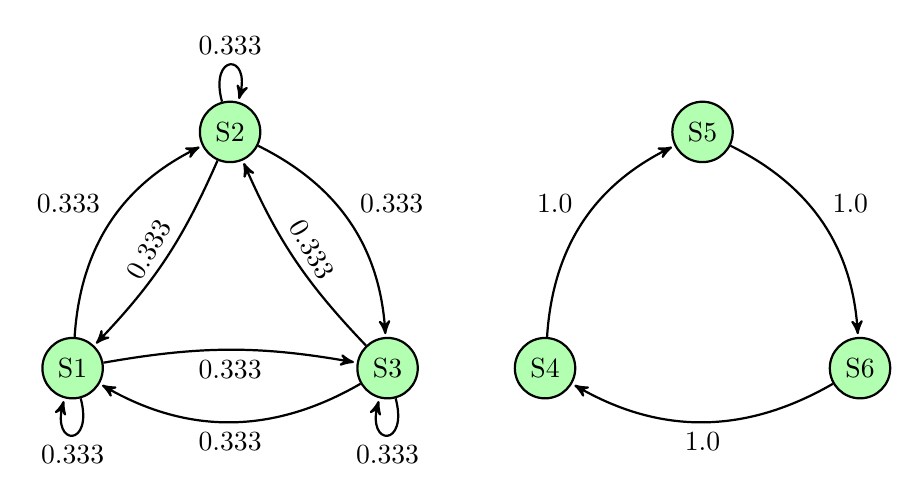
\begin{tikzpicture}[->,>=stealth',shorten >=1pt,auto,node distance=4cm,thick,main node/.style={circle,draw,font=\Large\bfseries}]
\tikzstyle{state} = [circle, draw=black, fill=green!30]
\tikzstyle{arrow} = [thick,->,>=stealth]

\node (s1) at (0,0) [state] {S1};
\node (s2) at (2,3) [state] {S2};
\node (s3) at (4,0) [state] {S3};
\node (s4) at (6,0) [state] {S4};
\node (s5) at (8,3) [state] {S5};
\node (s6) at (10,0) [state] {S6};

\path
    (s1) edge [loop below] node {0.333} (s1)
         edge [bend left] node {0.333} (s2)
         edge [bend left=10] node[below] {0.333} (s3)
    (s2) edge [loop above] node {0.333} (s2)
         edge [bend left=10] node[above,rotate=60] {0.333} (s1)
         edge [bend left] node {0.333} (s3)
    (s3) edge [loop below] node {0.333} (s3)
         edge [bend left=10] node[above,rotate=-60] {0.333} (s2)
         edge [bend left] node {0.333} (s1)
    (s4) edge [bend left] node {1.0} (s5)
    (s5) edge [bend left] node {1.0} (s6)
    (s6) edge [bend left] node {1.0} (s4);

\end{tikzpicture}
}
\end{figure}
\end{frame}

\begin{frame}
\frametitle{Results}
\begin{figure}[ht!]
        \centering
        \begin{minipage}[t]{0.45\textwidth}
                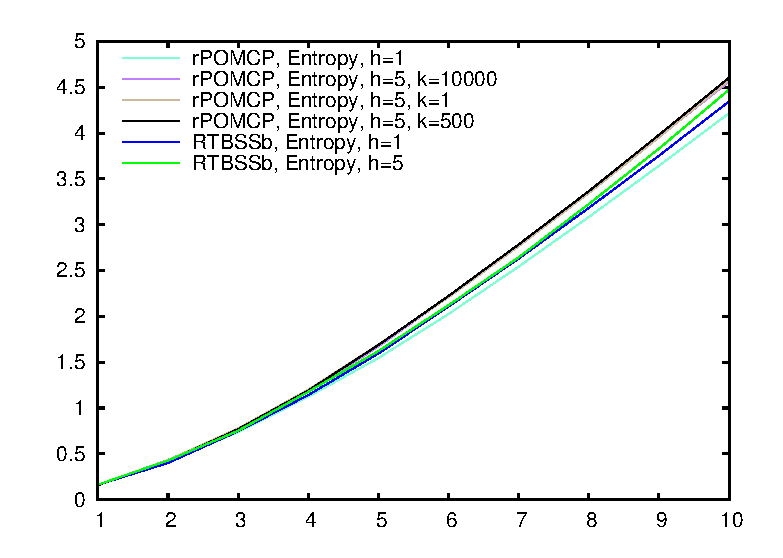
\includegraphics[width=\textwidth]{../images/Images/MyoResults/1e4/E/output}
                \caption{Results using 1e4 samples, with entropy as the reward function.}
                \label{fig:m4e}
        \end{minipage}%
        ~ %add desired spacing between images, e. g. ~, \quad, \qquad, \hfill etc.
          %(or a blank line to force the subfigure onto a new line)
        \begin{minipage}[t]{0.45\textwidth}
                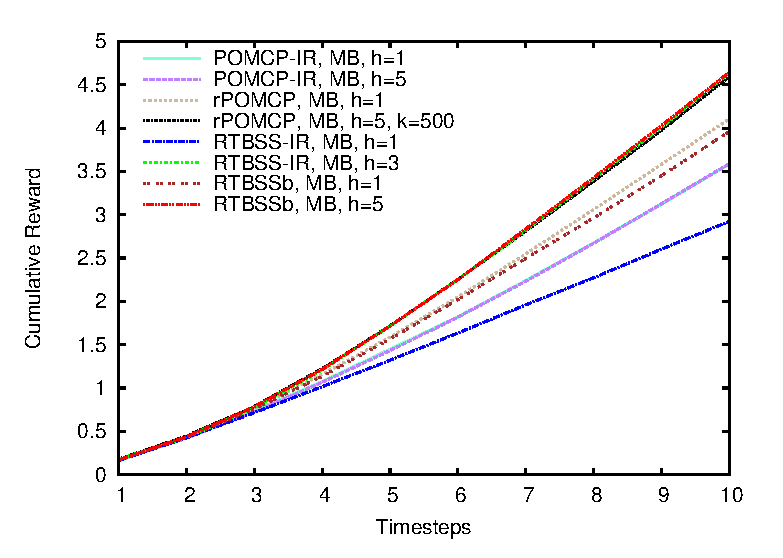
\includegraphics[width=\textwidth]{../images/Images/MyoResults/1e4/MB/output}
                \caption{Results using 1e4 samples, with max-of-belief as the reward function.}
                \label{fig:m5e}
        \end{minipage}
        \caption{Results in our first model, averaged over 3000 episodes.}
        \label{ref:myoentropyfig}
\end{figure}
\end{frame}

\subsection{Finite Budget}
\begin{frame}
    \frametitle{Finite Budget}

\begin{figure}[ht!]
\centering
\resizebox{!}{6cm}{%
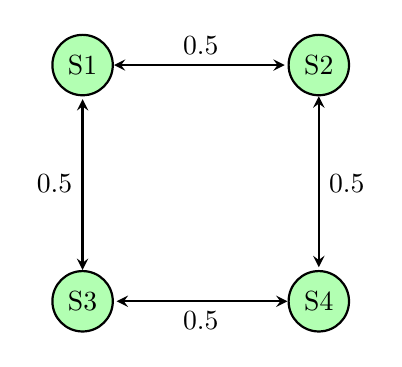
\begin{tikzpicture}[->,>=stealth',shorten >=1pt,auto,node distance=4cm,thick,main node/.style={circle,draw,font=\Large\bfseries}]
\tikzstyle{state} = [circle, draw=black, fill=green!30]
\tikzstyle{arrow} = [thick,<->,>=stealth]

\node (s1) at (0,3) [state] {S1};
\node (s2) at (3,3) [state] {S2};
\node (s3) at (0,0) [state] {S3};
\node (s4) at (3,0) [state] {S4};

\path
    (s1) edge [arrow] node {0.5} (s2)
    (s2) edge [arrow] node {0.5} (s4)
    (s3) edge [arrow] node {0.5} (s1)
    (s4) edge [arrow] node {0.5} (s3);

\end{tikzpicture}
}
\label{ref:finbudget1}
\end{figure}
\end{frame}

\begin{frame}
    \frametitle{Results}

\begin{figure}[ht!]
        \centering
        \begin{minipage}[t]{0.45\textwidth}
                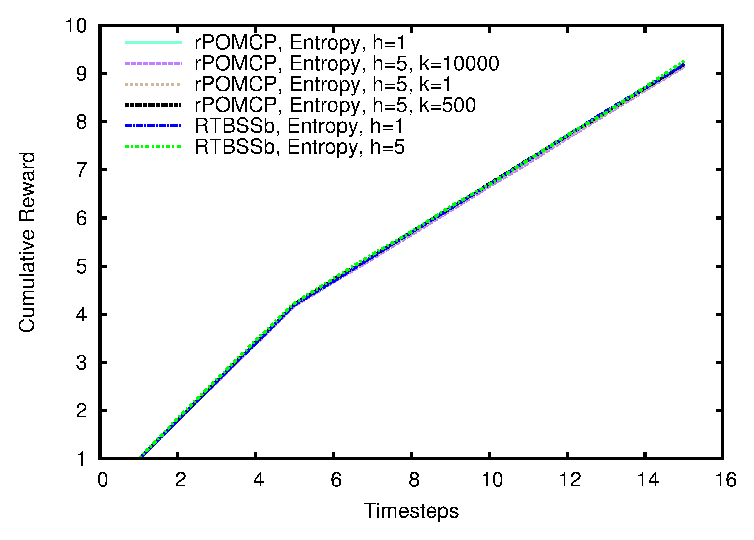
\includegraphics[width=\textwidth]{../images/Images/FiniteBudgetResults/0.5/1e4/E/output}
                \caption{Results using 1e4 samples, and entropy as the reward function.}
                \label{fig:fb4e5}
        \end{minipage}%
        ~ %add desired spacing between images, e. g. ~, \quad, \qquad, \hfill etc.
          %(or a blank line to force the minipage onto a new line)
        \begin{minipage}[t]{0.45\textwidth}
                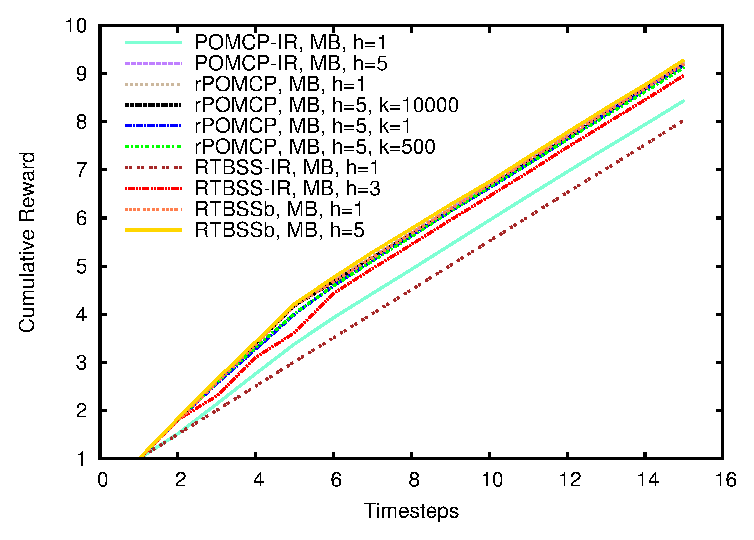
\includegraphics[width=\textwidth]{../images/Images/FiniteBudgetResults/0.5/1e4/MB/output}
                \caption{Results using 1e4 samples, and max-of-belief as the reward function.}
                \label{fig:fb5e5}
        \end{minipage}
        \caption{Results in the Finite Budget model with a transition factor of 0.5, averaged over 3000 episodes.}
        \label{ref:fbentropyfig5}
\end{figure}
\end{frame}

\begin{frame}
    \frametitle{Results}

\begin{figure}[ht!]
        \centering
        \begin{minipage}[t]{0.45\textwidth}
                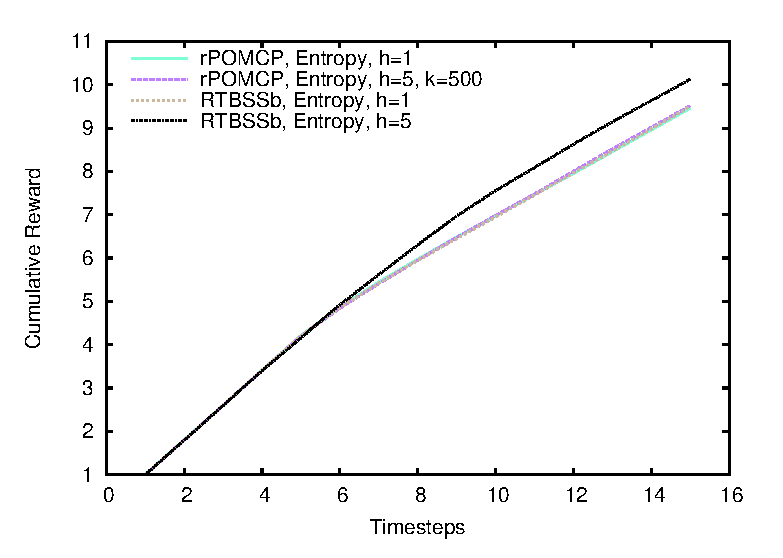
\includegraphics[width=\textwidth]{../images/Images/FiniteBudgetResults/0.75/1e4/E/output}
                \caption{Results using 1e4 samples, and entropy as the reward function.}
                \label{fig:fb4e75}
        \end{minipage}%
        ~ %add desired spacing between images, e. g. ~, \quad, \qquad, \hfill etc.
          %(or a blank line to force the minipage onto a new line)
        \begin{minipage}[t]{0.45\textwidth}
                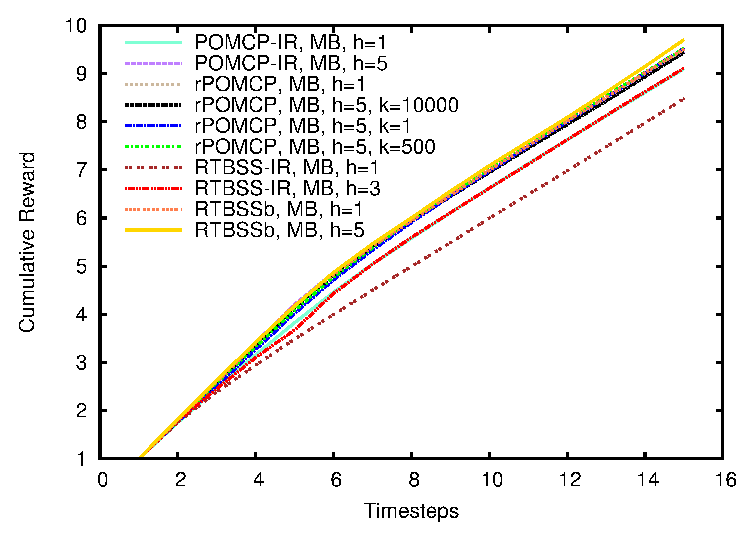
\includegraphics[width=\textwidth]{../images/Images/FiniteBudgetResults/0.75/1e4/MB/output}
                \caption{Results using 1e4 samples, and max-of-belief as the reward function.}
                \label{fig:fb5e75}
        \end{minipage}
        \caption{Results in the Finite Budget model with a transition factor of 0.75, averaged over 3000 episodes.}
        \label{ref:fbentropyfig75}
\end{figure}
\end{frame}

\subsection{Large Grid}
\begin{frame}
    \frametitle{Large Grid}
    \begin{block}{}
        Grid of either 20x20 or 50x50 cells. \\~\\
        Cameras observe non-overlapping 5x5 patches, imperfectly. \\~\\
        Targets are followed for 75 timesteps. \\~\\
        Multi-trackig achieved by parallelizing $\rho$POMCP for each target. \\~\\
        Other methods cannot be applied as the state space is too large.
    \end{block}
\end{frame}

\begin{frame}
    \frametitle{Multi Target Results}

\begin{figure}[ht]
        \centering
        \begin{minipage}[t]{0.5\textwidth}
                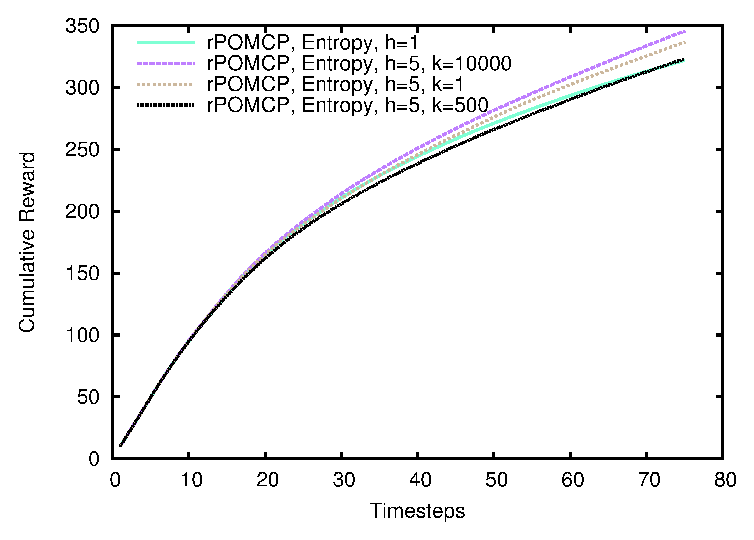
\includegraphics[width=\textwidth]{../images/Images/CameraPathResults/Big_50x50/Multi/E/output}
                \caption{Results using 1e4 samples and entropy.}
                \label{fig:cpb4e10}
        \end{minipage}%
        ~ %add desired spacing between images, e. g. ~, \quad, \qquad, \hfill etc.
          %(or a blank line to force the minipage onto a new line)
        \begin{minipage}[t]{0.5\textwidth}
                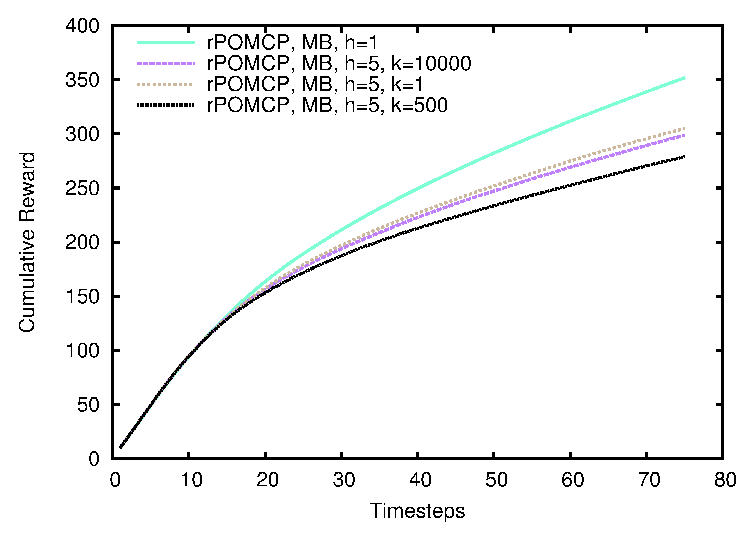
\includegraphics[width=\textwidth]{../images/Images/CameraPathResults/Big_50x50/Multi/MB/output}
                \caption{Results using 1e4 samples and max-of-belief.}
                \label{fig:cpb5mb10}
        \end{minipage}
        \caption{Results in the Large Grid 50x50 tracking 10 unique targets, averaged over 3000 episodes.}\label{fig:cpb10}
\end{figure}
\end{frame}

%------------------------------------------------

\begin{frame}
\frametitle{Videos}
\centerline{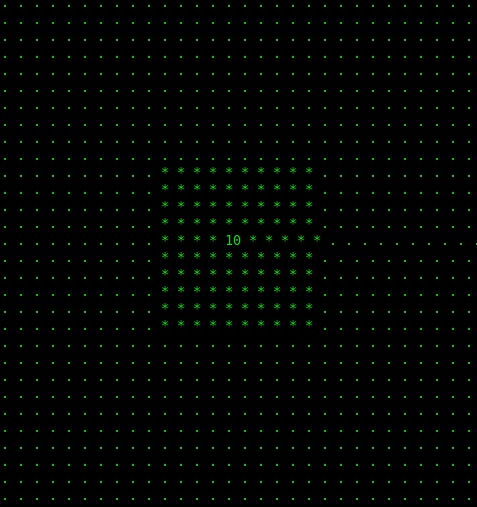
\includegraphics[width=5cm, height=5cm]{images/startvideo.png}}
\vspace{.75cm}
\begin{columns}[c] % The "c" option specifies centered vertical alignment while the "t" option is used for top vertical alignment
\column{.5\textwidth} % Right column and width
\centerline{\movie[externalviewer]{Entropy}{videos/entropy-10.ogv}}
\column{.5\textwidth} % Right column and width
\centerline{\movie[externalviewer]{Max of Belief}{videos/maxbelief-10.ogv}}
\end{columns}
\end{frame}

%----------------------------------------------------------------------------------------

\begin{frame}
\Huge{\centerline{The End}}
\end{frame}

%------------------------------------------------

\end{document}
